
\graphicspath{{./fig_shc1d/}}

\subsection{一次元定常熱伝導問題}

%
\subsubsection{目的}
本例題は,組み込み例題SHC1Dで,一次元の定常熱伝導問題を三次元モデルを用いて解析することにより,拡散項のコード部分の動作検証と予測精度を明らかにする.また,陰解法の収束挙動を陽解法と比較する.本例題は逐次実行のみで,問題サイズが小さくキャッシュサイズ内に収まるので性能評価は対象外とする.

%
\subsubsection{問題の定義と厳密解}
一次元の定常熱伝導問題は,\textbf{図\ref{fig:HC1D}}に示すような片持ちはりの熱伝導問題である~\cite{pat:91}.
壁面に取り付けられた断面積一定の放熱フィンで,壁面側は等温条件でもう一端は断熱条件となる.
はり自体は周囲流体へ熱伝達により放熱する.

\begin{figure}[htdp]
\begin{center}
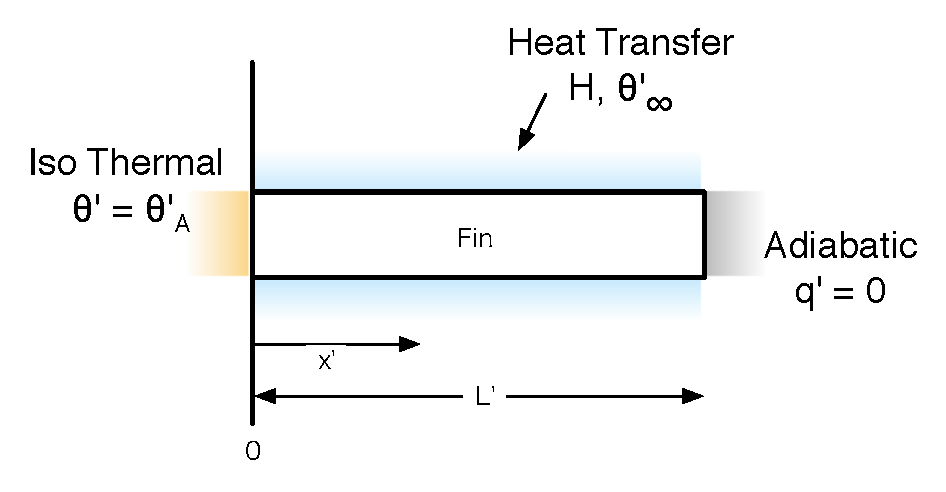
\includegraphics[width=9cm,clip]{1DHC.eps}
\end{center}
\caption{一次元定常熱伝導問題の模式図}
\label{fig:HC1D}
\end{figure}

問題の定式化としては\textbf{式(\ref{eq:shc1d gov eq})}の定常一次元熱伝導の形式となる.
支配方程式は,
\begin{equation}
\frac{d}{d{x}^{\prime}} \left({ \lambda \frac{d \theta^{\prime}}{d{x}^{\prime}} }\right) \,+\,\frac{H P^{\prime}}{A^{\prime}} \left({ {\theta_{\infty}}^{\prime} \,{-}\, \theta^{\prime} }\right)
\,{=}\,{0}
\label{eq:shc1d gov eq}
\end{equation}

\noindent $P',\,A'\,H,\,\lambda$は棒の周囲長さと断面積,熱伝達率,熱伝導率である.
\textbf{式(\ref{eq:shc1d gov eq})}の厳密解は,次式のようになる.
\begin{equation}
\theta
\,=\,
\frac{\theta^{\prime}\,-\,{\theta_{\infty}}^{\prime}} {{\theta_{A}}^{\prime}\,-\,{\theta_{\infty}}^{\prime}}
\,=\,
\frac{\cosh\left[{m\left({{L}{-}{x}}\right)}\right]}{\cosh\left({mL}\right)}{,}
\qquad m\,=\,\sqrt{\frac{H P^{\prime}}{\lambda A^{\prime}}}
\label{eq:1DHE exact solution}
\end{equation}


格子幅が$\Delta x^{\prime}=0.2$の場合には,厳密解のパラメータは,$H=12,\,L^{\prime}=1,\,{\theta_{A}}^{\prime}=200,\,{\theta_{\infty}}^{\prime}=100,\,\lambda=50,\,P^{\prime}=4\Delta x^{\prime},\,A^{\prime}={\Delta x^{\prime}}^2$として計算する.

\paragraph{領域設定}
計算領域は\textbf{図\ref{fig:shc1d dimension}}に示すようにx軸方向に放熱フィンをとり,y,z方向には5つだけセルを設ける.
領域の設定情報として,x方向の分割数をimaxにより与える.
放熱フィンを5分割したい場合には,imax=7を設定する.
$\mathrm{jmax=kmax=5}$で固定である.
このとき,格子幅は$\Delta x = \Delta y = \Delta z = 1\slash \mathrm{(imax-2)}$となる.
計算領域は,$[-\Delta x \sim (\mathrm{imax-1})\Delta x,\, -2.5\Delta y \sim 2.5\Delta y,\,-2.5\Delta z \sim 2.5\Delta z]$となる.

\begin{figure}[htdp]
\begin{center}
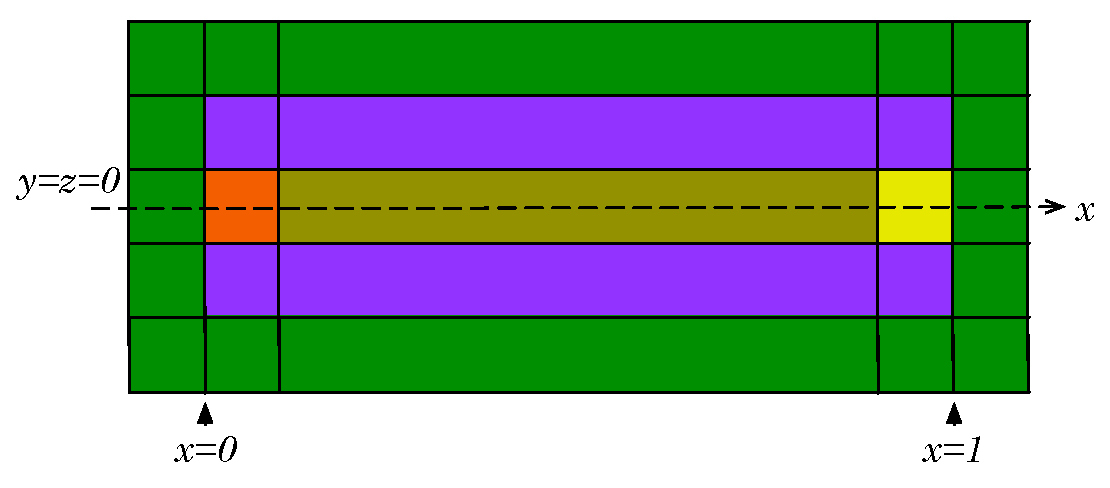
\includegraphics[width=8cm,clip]{dimension.eps}
\end{center}
\caption{計算領域の設定.色は\textbf{表\ref{tbl:set voxel ID}}に対応する.}
\label{fig:shc1d dimension}
\end{figure}

%
\pagebreak
\subsubsection{計算環境}
本計算に利用した計算機環境とソフトウェアを\textbf{表\ref{tbl: shc1d env}}に示す.

\begin{table}[htdp]
\small
\caption{計算機環境および利用ソフトウェア}
\begin{center}
\begin{tabular}{ll}\toprule
Computer & MacBook Pro\\
CPU & Intel Core i7 (2 Cores/CPU)\\
Clock & 2.66 GHz\\
Memory & 8GB\\
Cache(2nd) & 256 KB(each core)\\
Cache(3rd) & 4MB\\ 
OS & Mac OS X 10.6.5\\ \hline
MPI & OpenMPI 1.3.3\\
V-Sphere & ver. 1.8.2\\
CBC & ver. 1.3.0\\
FlowBase & ver. 2.3.0\\ \hline
Compiler & Intel Compiler Composer XE(12.0) C++/Fortran\\
Compile Option & -O3\\
\bottomrule
\end{tabular}
\end{center}
\label{tbl: shc1d env}
\end{table}


%
\subsubsection{解析モデルと計算パラメータ}

本例題は一次元の問題として解けますが,\textbf{図\ref{fig:HC model}}に示すように三次元で計算モデル作成し,三次元非定常熱伝導問題として解く.
この例題は固体熱伝導なので,流体セルは計算しない.

\begin{figure}[htdp]
\begin{minipage}{0.47\hsize}
\begin{center}
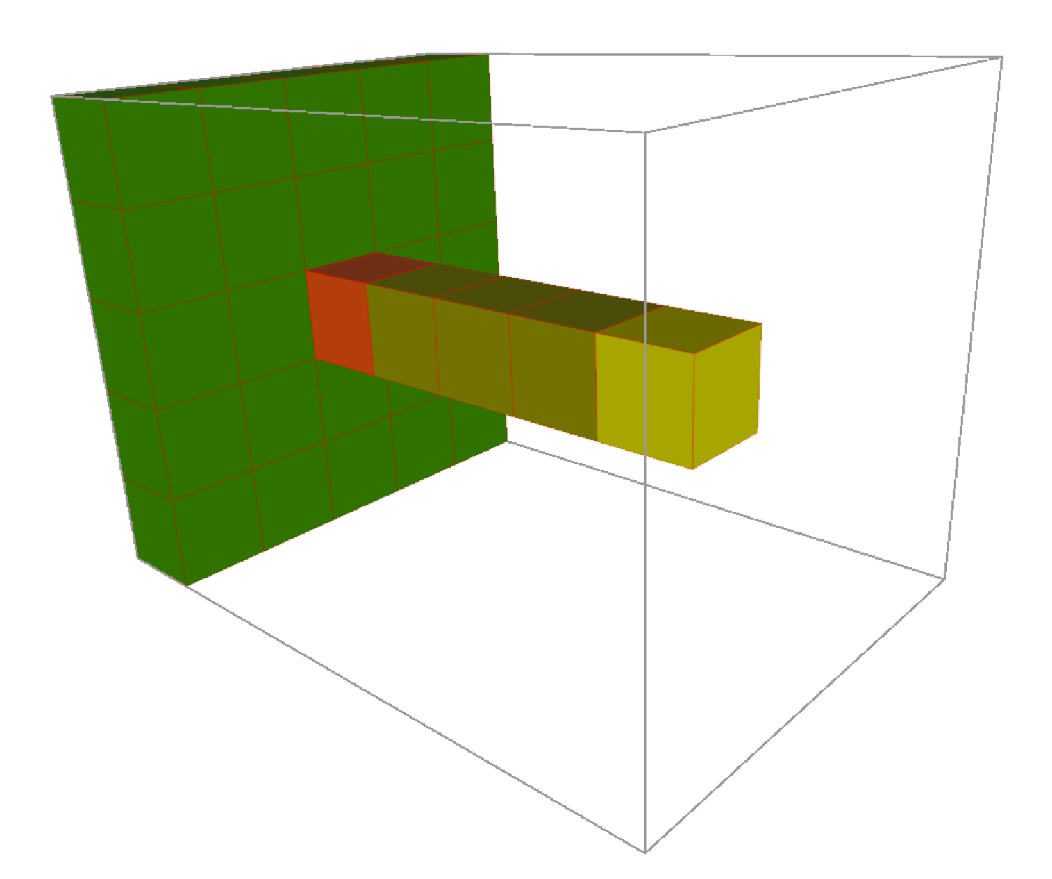
\includegraphics[height=5cm,clip]{model_iso.eps}
\end{center}
\end{minipage}
\begin{minipage}{0.47\hsize}
\begin{center}
\includegraphics[height=5cm,clip]{model_cross.eps}
\end{center}
\end{minipage}
\caption{一次元熱伝導問題を計算するための片持ち梁の三次元モデルとセルID (分割数が$7\times5\times5$の場合)}
\label{fig:HC model}
\end{figure}

計算モデルのセルIDは\textbf{表\ref{tbl:set voxel ID}}のように設定している.

\begin{table}[htdp]
\small
\caption{モデル作成時のID設定}
\begin{center}
\begin{tabular}{llll} \toprule
ID & Color & Medium & Property\\ \midrule
1 & Purple & Fluid & Water\\
500 & Orange & Solid & Iso-thermal wall\\
520 & Yellow & Solid & Adiabatic\\
600 & Green & Solid & Inactive cell\\
610 & Khaki & Solid & Heat conductor\\ \bottomrule
\end{tabular}
\end{center}
\label{tbl:set voxel ID}
\end{table}

計算に用いた物性値を\textbf{表\ref{tbl:shc1d medium_tbl}}に示す.
使用した物性値は物理的なものではなく,無次元のスケールアナリシスから導いた値である.
流体の物性値は実際には使用していない.
XMLパラメータファイルで,問題の指定単位を有次元,温度の単位にCelsiusを指定する.
計算終了時刻は定常状態までの時刻を見て設定している.

{\small
\begin{program}
<Elem name="Unit">
  <Param name="Unit_of_input_parameter" dtype="STRING" value="Dimensional" />
  <Param name="Temperature"             dtype="STRING" value="Celsius" />
</Elem>
\end{program}
}

\begin{table}[htdp]
\small
\caption{計算に用いた物性値}
\begin{center}
\begin{tabular}{llll}\\ \toprule
物性値 & & 流体(ID=1) & 固体(Others)\\ \midrule
密度 & $[kg/m^3]$ & $1.0$ & $1.0$\\
定圧比熱 & $[kJ/(kg K)]$ & $1.0$ & $1.0$\\
熱伝導率 & $[W/(m K)]$ & $1.0$ & $50.0$\\
動粘性係数 & $[m^2/s]$ & $1.0$ &\\
粘性係数 & $[Pa\,s]$ & $1.0$ &\\
音速 & $[m/s]$ & $1.0$ &\\
体膨張率 & $[1/K]$ & $1.0$ &\\ 
\bottomrule
\end{tabular}
\end{center}
\label{tbl:shc1d medium_tbl}
\end{table}


\paragraph{サンプリングの指定}
値のサンプリングは,$y=0,\, z=0$軸上の$x=0.0\sim 1.0$の範囲を分割してサンプリングする.



%
\subsubsection{計算結果と厳密解の比較}

\textbf{図\ref{fig:shc1d compare0}}に$\Delta x=0.2$の場合の無次元化した厳密解と計算結果の比較結果を示す.
5セルの近似であるが,厳密解との誤差は最大2\%であることがわかる.

\begin{figure}[htbp]
\begin{minipage}{.47\textwidth}
\begin{center}
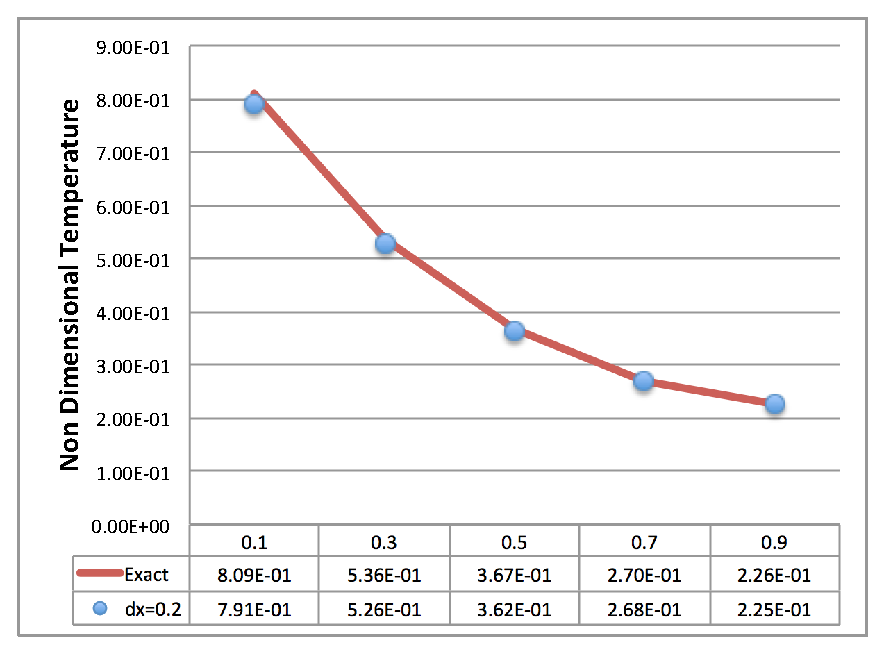
\includegraphics[width=8cm,clip]{cmp_0.eps}
\end{center}
\caption{厳密解と計算結果の比較(Euler陽解法,$\Delta x=0.2 m,\,\Delta t=4.0\times 10^{-4} sec.$, $t=2.48\times 10^{-2} sec.$)}
\label{fig:shc1d compare0}
\end{minipage} \hfill
\begin{minipage}{.47\textwidth}
\begin{center}
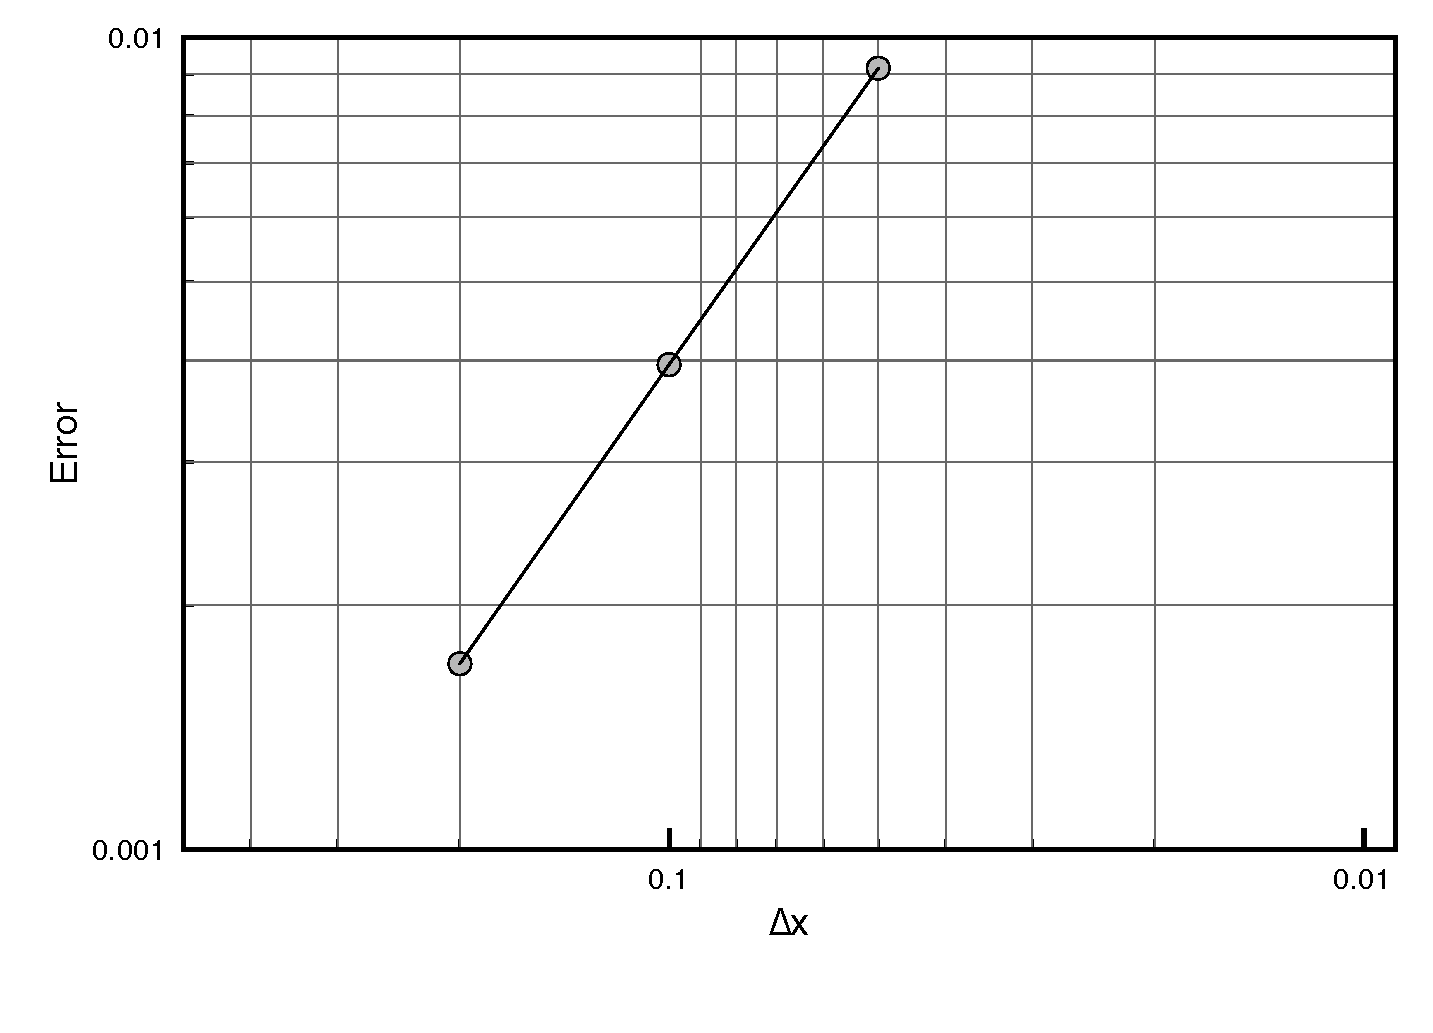
\includegraphics[width=8cm,clip]{error.eps}
\end{center}
\caption{計算結果の格子依存性の比較 ($y=ax^b,\,b=1.21$)}
\label{fig:shc1d compare1}
\end{minipage}
\end{figure}

\textbf{図\ref{fig:shc1d compare1}}には,誤差のメッシュ依存性を示す.グラフの傾きから誤差は格子幅の変化量に対して1.2倍の割合で減少していることがわかる.つまり,この問題の場合には予測精度は1.2次となっている.拡散項のスキームは空間二次精度で離散化されており空間2次精度が期待されるが,境界条件の影響により近似精度が低下している.つまり,等温境界と熱伝達境界の近似精度が一次であるので,この部分の影響を強く受けている.

陽解法では$\Delta t$の値を変化させ,拡散数$D=\lambda \Delta t \slash {\Delta x}^2<1\slash 2$の範囲で安定に計算でき,$D>1\slash 2$では不安定になり発散すること,陰解法では$D\sim 1$程度まで安定に計算できることが確認できる.

%
\pagebreak
\subsubsection{ファイルのメモ}

例題の添付ファイルの説明を以下に示す.ただし,Euler陰解法は$\Delta x=0.2$の場合のみである.

\begin{quote}
\begin{tabbing}
\hspace{18em}\= \hspace{20em}\kill
shc1d\_ee\_\{005, 01, 02\}.xml \> Euler陽解法$\Delta x=0.05,\,0.1,\,0.2$のパラメータ\\
shc1d\_ei\_02.xml \> Euler陰解法$\Delta x=0.2$のパラメータ\\
condition\_*\_\{005, 01, 02\}.txt \> conditionファイル(*=ee:Euler陽解法,ei:Euler陰解法)\\
history\_base\_*\_\{005, 01, 02\}.txt \> history\_baseファイル\\
history\_compo\_*\_\{005, 01, 02\}.txt \> history\_compoファイル\\
sampling\_*\_\{005, 01, 02\}.txt \> samplingファイル\\
comparison.xlsx \> \textbf{図\ref{fig:shc1d compare0}}と\textbf{図\ref{fig:shc1d compare1}}の結果のファイル\\
exact.py \> 厳密解を計算するスクリプトファイル\\
Error.plot \> plotファイル(http://plot.micw.eu/)\\
\end{tabbing}
\end{quote}

\paragraph{厳密解の計算}
exact.pyをエディタで開き,分割数nの値を変更する.実行は以下のようにコマンドラインでタイプすると,対応する結果が表示される.1カラム目がx座標,2カラム目が厳密解である.
{ \small
\begin{program}
$ python exact.py

0.1 0.808704519533
0.3 0.535692813577
0.5 0.367190344487
0.7 0.270323674338
0.9 0.22619491703
\end{program}
}

